\documentclass[notes,11pt, aspectratio=169]{beamer}

\usepackage{pgfpages}
% These slides also contain speaker notes. You can print just the slides,
% just the notes, or both, depending on the setting below. Comment out the want
% you want.
\setbeameroption{hide notes} % Only slide
%\setbeameroption{show only notes} % Only notes
%\setbeameroption{show notes on second screen=right} % Both

%\usepackage[scaled=1.0]{helvet}
\usepackage{array}

\usepackage{graphicx}
\usepackage{tikz}
\usetikzlibrary{calc}
\usetikzlibrary{matrix}
\usetikzlibrary{positioning}

\newcommand{\payoff}[4][below]{\node[#1]at(#2){$(#3,#4)$};}
\usepackage{verbatim}
\setbeamertemplate{note page}{\pagecolor{gray!5}\insertnote}
\usetikzlibrary{positioning}
\usetikzlibrary{snakes}
\usetikzlibrary{calc}
\usetikzlibrary{arrows}
\usetikzlibrary{decorations.markings}
\usetikzlibrary{shapes.misc}
\usetikzlibrary{matrix,shapes,arrows,fit,tikzmark}
\usepackage{amsmath}
\usepackage{mathpazo}
\usepackage{hyperref}
\usepackage{lipsum}
\usepackage{multimedia}
\usepackage{graphicx}
\usepackage{multirow}
\usepackage{graphicx}
\usepackage{dcolumn}
\usepackage{bbm}
\newcolumntype{d}[0]{D{.}{.}{5}}

\usepackage{changepage}
\usepackage{appendixnumberbeamer}
\newcommand{\beginbackup}{
   \newcounter{framenumbervorappendix}
   \setcounter{framenumbervorappendix}{\value{framenumber}}
   \setbeamertemplate{footline}
   {
     \leavevmode%
     \hline
     box{%
       \begin{beamercolorbox}[wd=\paperwidth,ht=2.25ex,dp=1ex,right]{footlinecolor}%
%         \insertframenumber  \hspace*{2ex} 
       \end{beamercolorbox}}%
     \vskip0pt%
   }
 }
\newcommand{\backupend}{
   \addtocounter{framenumbervorappendix}{-\value{framenumber}}
   \addtocounter{framenumber}{\value{framenumbervorappendix}} 
}


\usepackage{graphicx}
\usepackage[space]{grffile}
\usepackage{booktabs}

% These are my colors -- there are many like them, but these ones are mine.
\definecolor{blue}{RGB}{0,114,178}
\definecolor{red}{RGB}{213,94,0}
\definecolor{yellow}{RGB}{240,228,66}
\definecolor{green}{RGB}{0,158,115}

\hypersetup{
  colorlinks=false,
  linkbordercolor = {white},
  linkcolor = {blue}
}

\usepackage{graphicx,stackengine,xcolor}
\newcommand\Circle[1]{%
	\def\useanchorwidth{T}%
	\def\stacktype{L}%
	\stackon[0pt]{#1}{\scalebox{2.0}[1.15]{\textcolor{red}{$\bigcirc$}}}%
}

%% I use a beige off white for my background
\definecolor{MyBackground}{RGB}{255,253,218}

%% Uncomment this if you want to change the background color to something else
%\setbeamercolor{background canvas}{bg=MyBackground}

%% Change the bg color to adjust your transition slide background color!
\newenvironment{transitionframe}{
  \setbeamercolor{background canvas}{bg=white}
  \begin{frame}}{
    \end{frame}
}

\setbeamercolor{frametitle}{fg=blue}
\setbeamercolor{title}{fg=black}
\setbeamertemplate{footline}[frame number]
\setbeamertemplate{navigation symbols}{} 
\setbeamertemplate{itemize items}{-}
\setbeamercolor{itemize item}{fg=blue}
\setbeamercolor{itemize subitem}{fg=blue}
\setbeamercolor{enumerate item}{fg=blue}
\setbeamercolor{enumerate subitem}{fg=blue}
\setbeamercolor{button}{bg=MyBackground,fg=blue,}

%%% TIKZ STUFF
\tikzset{   
	every picture/.style={remember picture,baseline},
	every node/.style={anchor=base,align=center,outer sep=1.5pt},
	every path/.style={thick},
}
\newcommand\marktopleft[1]{%
	\tikz[overlay,remember picture] 
	\node (marker-#1-a) at (-.3em,.3em) {};%
}
\newcommand\markbottomright[2]{%
	\tikz[overlay,remember picture] 
	\node (marker-#1-b) at (0em,0em) {};%
}
\tikzstyle{every picture}+=[remember picture] 
\tikzstyle{mybox} =[draw=black, very thick, rectangle, inner sep=10pt, inner ysep=20pt]
\tikzstyle{fancytitle} =[draw=black,fill=red, text=white]
%%%% END TIKZ STUFF


% If you like road maps, rather than having clutter at the top, have a roadmap show up at the end of each section 
% (and after your introduction)
% Uncomment this is if you want the roadmap!
% \AtBeginSection[]
% {
%    \begin{frame}
%        \frametitle{Roadmap of Talk}
%        \tableofcontents[currentsection]
%    \end{frame}
% }
\setbeamercolor{section in toc}{fg=blue}
\setbeamercolor{subsection in toc}{fg=red}
\setbeamersize{text margin left=1em,text margin right=1em} 

\newenvironment{wideitemize}{\itemize\addtolength{\itemsep}{10pt}}{\enditemize}
\newenvironment{wideenumerate}{\enumerate\addtolength{\itemsep}{10pt}}{\endenumerate}

\usepackage{environ}
\NewEnviron{videoframe}[1]{
  \begin{frame}
    \vspace{-8pt}
    \begin{columns}[onlytextwidth, T] % align columns
      \begin{column}{.58\textwidth}
        \begin{minipage}[t][\textheight][t]
          {\dimexpr\textwidth}
          \vspace{8pt}
          \hspace{4pt} {\Large \sc \textcolor{blue}{#1}}
          \vspace{8pt}
          
          \BODY
        \end{minipage}
      \end{column}%
      \hfill%
      \begin{column}{.42\textwidth}
        \colorbox{green!20}{\begin{minipage}[t][1.2\textheight][t]
            {\dimexpr\textwidth}
            Face goes here
          \end{minipage}}
      \end{column}%
    \end{columns}
  \end{frame}
}

\title[]{\textcolor{blue}{ECN 453: Collusion and Price Wars 1}}
\author[PGP]{}
\institute[FRBNY]{\small{\begin{tabular}{c c c}
Nicholas Vreugdenhil \\
\end{tabular}}}
\date{} 

\begin{document}

% Title Slide
\begin{frame}
\maketitle
  \centering
\end{frame}

% INTRO

\begin{frame}{Collusion and Price Wars: Motivation}
\begin{wideitemize}
	\item Adam Smith: ``People of the same trade seldom meet together, even for merriment and diversion, but the conversation ends in a conspiracy against the public, or in some contrivance to raise prices''.
\end{wideitemize}
\begin{figure}
	\centering
	\includegraphics[scale=0.3]{handshake.jpg}
\end{figure}
\end{frame}

\begin{frame}{Collusion and Price Wars: Motivation}
	\begin{wideitemize}
		\item Competition creates an \textbf{externality}: 
		\begin{wideitemize}
			\item e.g. Consider Cournot: firms maximize their own profit not accounting that part of the increase in profits is coming at the expense of the other firms in the market.
		\end{wideitemize}
		\item Firms could do better by establishing agreement between themselves to increase their \textbf{market power}.
		\item These agreements are generically referred to as \textbf{collusion}.
		\begin{wideitemize}
			\item Organized cartels
			\item Secret agreements
			\item Tacit agreements
		\end{wideitemize}
		\item In this part of the course we will discuss these practices in detail. 
	\end{wideitemize}
\end{frame}


\begin{frame}{Collusion and Price Wars: Motivation}
	\begin{wideitemize}
		\item Types of agreement
		\begin{wideitemize}
			\item Increase price
			\item Decrease quantity
			\item Territory agreements
			\item Agreements about quality, advertising etc
		\end{wideitemize}
		\item Key to many agreements: \textbf{dynamic considerations}
		\begin{wideitemize}
			\item `Dynamic' means agreements with a time dimension. E.g. `Let's set the monopoly price together today otherwise I'll punish you tomorrow'.
		\end{wideitemize}
		\item So, before talking about collusive agreements, we first need to understand how to solve games/strategic interactions with dynamics (\textbf{repeated games}).
	\end{wideitemize}
\end{frame}

\begin{frame}{Plan}
	\begin{wideenumerate}
		\item Present discounted value
		\item Repeated games: method
		\item Stability of collusive agreements
	\end{wideenumerate}
\end{frame}

\begin{frame}{Plan}
	\begin{wideenumerate}
		\item \textbf{Present discounted value}
		\item Repeated games: method
		\item Stability of collusive agreements
	\end{wideenumerate}
\end{frame}

\begin{frame}{Present discounted value}
	\begin{wideitemize}
		\item First need to introduce the idea of a \textbf{discount factor}, denoted $\delta$
		\item Discount factor $\delta \in [0, 1]$. Idea: how much you value getting \$1 in the next period vs  getting \$1 now.
		\begin{wideitemize}
			\item $\delta = 0$: \pause don't value the future at all
			\item $\delta = 1$: \pause value \$1 next period the same as \$1 today (e.g. don't care about waiting)
			\item $0 < \delta < 1$: e.g. $\delta = 0.9$ value \$1 in the next period as 90c today.
		\end{wideitemize}
	\end{wideitemize}
\end{frame}


\begin{frame}{Present discounted value}
	\begin{wideitemize}
		\item \textbf{Question}: What is the \textbf{present discounted value} of receiving \$5 repeatedly in every period (where there are infinite periods) if the discount factor is $\delta < 1$?
		\item Value = $5 + \delta 5 + \delta^2 5 + ...$
		\begin{wideitemize}
			\item Why is the $\delta$ squared in the third term on the right-hand-side? \pause 
			\item A: This is the value two periods in the future, so multiply it once to discount it back to one period in the future, and discount it again to get it back to the current period.
		\end{wideitemize}
		\item \textbf{Important math equation}: (Geometric sum:)
		\begin{wideitemize}
			\item Constant: c
			\item Discount value: $\delta < 1$ then:
			\begin{align*}
				c + \delta c + \delta^2 c + \delta^3 c + ... = \frac{c}{1-\delta}
			\end{align*}
		\end{wideitemize}
		\item So, overall, Value = $\frac{c}{1-\delta}$
	\end{wideitemize}
\end{frame}

\begin{frame}{Plan}
	\begin{wideenumerate}
		\item Present discounted value
		\item \textbf{Repeated games: method}
		\item Stability of collusive agreements
	\end{wideenumerate}
\end{frame}

\begin{frame}{Repeated games: prisoner's dilemma with $T=1$}
	\begin{columns}[onlytextwidth, T] 
		\begin{column}{.55\textwidth}
			\begin{wideitemize}
				\item Denote $T$ as number of times the game is repeated. Here, consider $T=1$.
				\item $(B,R)$ is the unique Nash equilibrium.
				\item Both firms would do much better if could somehow agree to play (T,L)
			\end{wideitemize}
		\end{column}
		\begin{column}{.45\textwidth}
			\vspace{20pt}
			\hspace{20pt}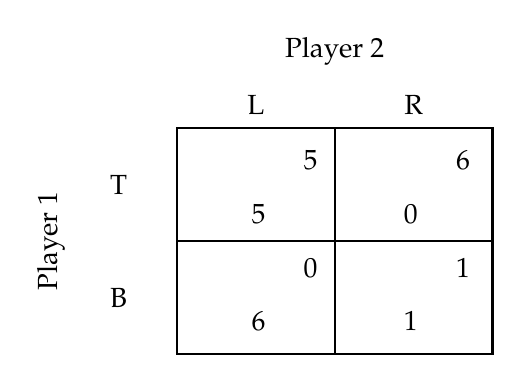
\begin{tikzpicture}
				\matrix[matrix of math nodes,
				every odd row/.style={align=right},every evenrow/.style={align=left},every node/.style={text width=1.5cm},row sep=0.2cm,column sep=0.2cm,ampersand replacement=\&] (m) {
					5\&6 \\
					5\&0 \\
					0 \&1 \\
					6 \&1\\
				};
				\draw (m.north east) rectangle (m.south west);
				\draw (m.north) -- (m.south);
				\draw (m.east) -- (m.west);
				
				% Player 1
				\coordinate (c) at ($(m.north west)!0.25!(m.south west)$);
				\coordinate (d) at ($(m.north west)!0.75!(m.south west)$);
				\node[left=2pt of c,text width=1cm]  {T};
				\node[left=2pt of d,text width=1cm]  {B};
				
				% Player 2
				\coordinate (a) at ($(m.north west)!0.25!(m.north east)$);
				\coordinate (b) at ($(m.north west)!0.75!(m.north east)$);
				\node[above=5pt of a,anchor=base] {L};
				\node[above=5pt of b,anchor=base] {R};
				
				\node[above=18pt of m.north] (firm b) {Player 2};
				\node[left=1.6cm of m.west,rotate=90,align=center,anchor=center] {Player 1};
				
				%\node[above=5pt of firm b]  {Payoff Matrix};
			\end{tikzpicture}
		\end{column}
	\end{columns}
\end{frame}


\begin{frame}{Repeated games: prisoner's dilemma with $T=2$}
	\begin{columns}[onlytextwidth, T] 
		\begin{column}{.55\textwidth}
			\begin{wideitemize}
				\item Strategies in repeated games: `contingent strategies'
				\begin{wideitemize}
					\item Contingent strategy: given all the actions in the previous periods (i.e, the history of actions), choose an action in the current period
				\end{wideitemize}
			\end{wideitemize}
		\end{column}
		\begin{column}{.45\textwidth}
			\vspace{20pt}
			\hspace{20pt}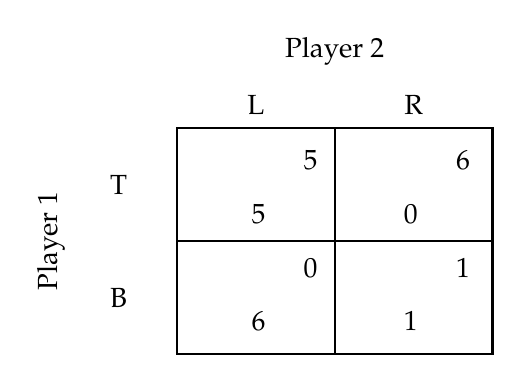
\begin{tikzpicture}
				\matrix[matrix of math nodes,
				every odd row/.style={align=right},every evenrow/.style={align=left},every node/.style={text width=1.5cm},row sep=0.2cm,column sep=0.2cm,ampersand replacement=\&] (m) {
					5\&6 \\
					5\&0 \\
					0 \&1 \\
					6 \&1\\
				};
				\draw (m.north east) rectangle (m.south west);
				\draw (m.north) -- (m.south);
				\draw (m.east) -- (m.west);
				
				% Player 1
				\coordinate (c) at ($(m.north west)!0.25!(m.south west)$);
				\coordinate (d) at ($(m.north west)!0.75!(m.south west)$);
				\node[left=2pt of c,text width=1cm]  {T};
				\node[left=2pt of d,text width=1cm]  {B};
				
				% Player 2
				\coordinate (a) at ($(m.north west)!0.25!(m.north east)$);
				\coordinate (b) at ($(m.north west)!0.75!(m.north east)$);
				\node[above=5pt of a,anchor=base] {L};
				\node[above=5pt of b,anchor=base] {R};
				
				\node[above=18pt of m.north] (firm b) {Player 2};
				\node[left=1.6cm of m.west,rotate=90,align=center,anchor=center] {Player 1};
				
				%\node[above=5pt of firm b]  {Payoff Matrix};
			\end{tikzpicture}
		\end{column}
	\end{columns}
\end{frame}


\begin{frame}{Repeated games: prisoner's dilemma with $T=2$}
	\begin{columns}[onlytextwidth, T] 
		\begin{column}{.55\textwidth}
			\begin{wideitemize}
				\item Is playing (B,R) in both periods a Nash equilibrium?
				\item \pause Yes! Are there any other equilibria? 
				\item Let's consider one alternative called the \textbf{grim trigger strategy}.
				\item Idea: play (T,L) . If there is \textbf{any} deviation then play (B,R).
			\end{wideitemize}
		\end{column}
		\begin{column}{.45\textwidth}
			\vspace{20pt}
			\hspace{20pt}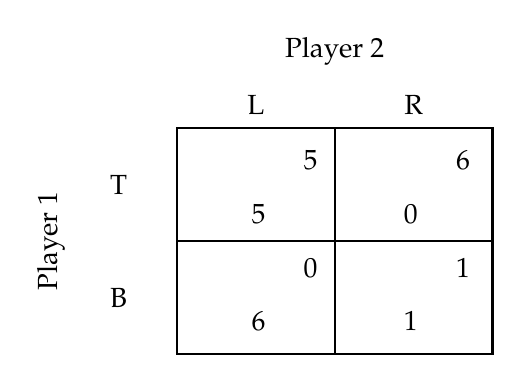
\begin{tikzpicture}
				\matrix[matrix of math nodes,
				every odd row/.style={align=right},every evenrow/.style={align=left},every node/.style={text width=1.5cm},row sep=0.2cm,column sep=0.2cm,ampersand replacement=\&] (m) {
					5\&6 \\
					5\&0 \\
					0 \&1 \\
					6 \&1\\
				};
				\draw (m.north east) rectangle (m.south west);
				\draw (m.north) -- (m.south);
				\draw (m.east) -- (m.west);
				
				% Player 1
				\coordinate (c) at ($(m.north west)!0.25!(m.south west)$);
				\coordinate (d) at ($(m.north west)!0.75!(m.south west)$);
				\node[left=2pt of c,text width=1cm]  {T};
				\node[left=2pt of d,text width=1cm]  {B};
				
				% Player 2
				\coordinate (a) at ($(m.north west)!0.25!(m.north east)$);
				\coordinate (b) at ($(m.north west)!0.75!(m.north east)$);
				\node[above=5pt of a,anchor=base] {L};
				\node[above=5pt of b,anchor=base] {R};
				
				\node[above=18pt of m.north] (firm b) {Player 2};
				\node[left=1.6cm of m.west,rotate=90,align=center,anchor=center] {Player 1};
				
				%\node[above=5pt of firm b]  {Payoff Matrix};
			\end{tikzpicture}
		\end{column}
	\end{columns}
\end{frame}

\begin{frame}{Repeated games: prisoner's dilemma with $T=2$}
	\begin{columns}[onlytextwidth, T] 
		\begin{column}{.55\textwidth}
			\begin{wideitemize}
				\item \textbf{Grim trigger strategy}:
				\begin{wideitemize}
					\item Idea: play (T,L) in period 1. 
					\item Threat: play (B,R) in period 2 contingent on either player deviating.  
					\item Otherwise, play (T,L) again.
					\item Is this a NE?
				\end{wideitemize}
			\end{wideitemize}
		\end{column}
		\begin{column}{.45\textwidth}
			\vspace{20pt}
			\hspace{20pt}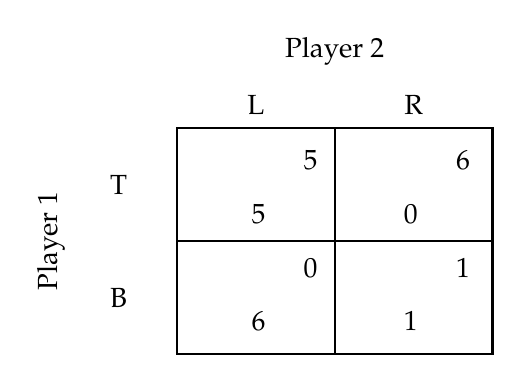
\begin{tikzpicture}
				\matrix[matrix of math nodes,
				every odd row/.style={align=right},every evenrow/.style={align=left},every node/.style={text width=1.5cm},row sep=0.2cm,column sep=0.2cm,ampersand replacement=\&] (m) {
					5\&6 \\
					5\&0 \\
					0 \&1 \\
					6 \&1\\
				};
				\draw (m.north east) rectangle (m.south west);
				\draw (m.north) -- (m.south);
				\draw (m.east) -- (m.west);
				
				% Player 1
				\coordinate (c) at ($(m.north west)!0.25!(m.south west)$);
				\coordinate (d) at ($(m.north west)!0.75!(m.south west)$);
				\node[left=2pt of c,text width=1cm]  {T};
				\node[left=2pt of d,text width=1cm]  {B};
				
				% Player 2
				\coordinate (a) at ($(m.north west)!0.25!(m.north east)$);
				\coordinate (b) at ($(m.north west)!0.75!(m.north east)$);
				\node[above=5pt of a,anchor=base] {L};
				\node[above=5pt of b,anchor=base] {R};
				
				\node[above=18pt of m.north] (firm b) {Player 2};
				\node[left=1.6cm of m.west,rotate=90,align=center,anchor=center] {Player 1};
				
				%\node[above=5pt of firm b]  {Payoff Matrix};
			\end{tikzpicture}
		\end{column}
	\end{columns}
\end{frame}

\begin{frame}{Repeated games: prisoner's dilemma with $T=2$}
	\begin{columns}[onlytextwidth, T] 
		\begin{column}{.55\textwidth}
			\begin{wideitemize}
				\item Check grim trigger strategy using backwards induction.
				\item At t=2: Always play (B,R)
				\item So, at t=1: cannot promise to play (T,L) in period 2 credibly.
				\item So, grim trigger is \textit{not} a Nash equilibrium in the $T=2$ game.
			\end{wideitemize}
		\end{column}
		\begin{column}{.45\textwidth}
			\vspace{20pt}
			\hspace{20pt}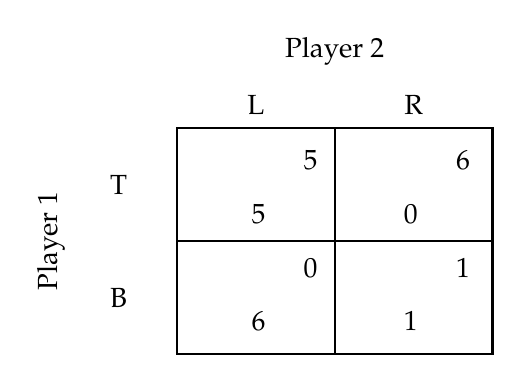
\begin{tikzpicture}
				\matrix[matrix of math nodes,
				every odd row/.style={align=right},every evenrow/.style={align=left},every node/.style={text width=1.5cm},row sep=0.2cm,column sep=0.2cm,ampersand replacement=\&] (m) {
					5\&6 \\
					5\&0 \\
					0 \&1 \\
					6 \&1\\
				};
				\draw (m.north east) rectangle (m.south west);
				\draw (m.north) -- (m.south);
				\draw (m.east) -- (m.west);
				
				% Player 1
				\coordinate (c) at ($(m.north west)!0.25!(m.south west)$);
				\coordinate (d) at ($(m.north west)!0.75!(m.south west)$);
				\node[left=2pt of c,text width=1cm]  {T};
				\node[left=2pt of d,text width=1cm]  {B};
				
				% Player 2
				\coordinate (a) at ($(m.north west)!0.25!(m.north east)$);
				\coordinate (b) at ($(m.north west)!0.75!(m.north east)$);
				\node[above=5pt of a,anchor=base] {L};
				\node[above=5pt of b,anchor=base] {R};
				
				\node[above=18pt of m.north] (firm b) {Player 2};
				\node[left=1.6cm of m.west,rotate=90,align=center,anchor=center] {Player 1};
				
				%\node[above=5pt of firm b]  {Payoff Matrix};
			\end{tikzpicture}
		\end{column}
	\end{columns}
\end{frame}

\begin{frame}{Repeated games: prisoner's dilemma with $T=\infty$}
	\begin{columns}[onlytextwidth, T] 
		\begin{column}{.55\textwidth}
			\begin{wideitemize}
			\item As before, playing $(B,R)$ every period is a Nash equilibrium.
			\item But now let's consider the grim trigger strategy again:
			\begin{wideitemize}
				\item Choose $(T,L)$ if the history has been $(T,L)$ for \textit{every} period in the past.
				\item Choose $(B,R)$ otherwise.
			\end{wideitemize}
			\item \textbf{Question:} Is the grim trigger strategy a Nash equilibrium?
	\end{wideitemize}
		\end{column}
		\begin{column}{.45\textwidth}
			\vspace{20pt}
			\hspace{20pt}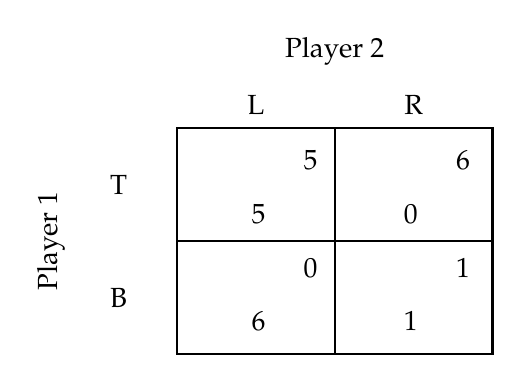
\begin{tikzpicture}
				\matrix[matrix of math nodes,
				every odd row/.style={align=right},every evenrow/.style={align=left},every node/.style={text width=1.5cm},row sep=0.2cm,column sep=0.2cm,ampersand replacement=\&] (m) {
					5\&6 \\
					5\&0 \\
					0 \&1 \\
					6 \&1\\
				};
				\draw (m.north east) rectangle (m.south west);
				\draw (m.north) -- (m.south);
				\draw (m.east) -- (m.west);
				
				% Player 1
				\coordinate (c) at ($(m.north west)!0.25!(m.south west)$);
				\coordinate (d) at ($(m.north west)!0.75!(m.south west)$);
				\node[left=2pt of c,text width=1cm]  {T};
				\node[left=2pt of d,text width=1cm]  {B};
				
				% Player 2
				\coordinate (a) at ($(m.north west)!0.25!(m.north east)$);
				\coordinate (b) at ($(m.north west)!0.75!(m.north east)$);
				\node[above=5pt of a,anchor=base] {L};
				\node[above=5pt of b,anchor=base] {R};
				
				\node[above=18pt of m.north] (firm b) {Player 2};
				\node[left=1.6cm of m.west,rotate=90,align=center,anchor=center] {Player 1};
				
				%\node[above=5pt of firm b]  {Payoff Matrix};
			\end{tikzpicture}
		\end{column}
	\end{columns}
\end{frame}

\begin{frame}{Repeated games: prisoner's dilemma with $T=\infty$}
	\begin{columns}[onlytextwidth, T] 
		\begin{column}{.55\textwidth}
			\begin{wideitemize}
				\item \textbf{Question:} Is the grim trigger strategy a Nash equilibrium?
				\item Equilibrium payoff:
				\item $\Pi = 5 + \delta 5 + \delta^2 5 + ... = \frac{5}{1-\delta}$
				\item Deviation payoff:
				\item $\Pi' = 6 + \underbrace{\delta 1 + \delta^2 1 + ... }_{\text{Grim trigger punishment}}= 6 + \frac{\delta}{1-\delta}$
				\item Is a NE if no incentive to deviate: $\Pi \geq \Pi'$
				\begin{wideitemize}
					\item Substitute in payoffs from above: $\delta \geq 1/5$
					\item Idea: if $\delta$ high enough, deviation doesn't pay.
				\end{wideitemize}
			\end{wideitemize}
		\end{column}
		\begin{column}{.45\textwidth}
			\vspace{20pt}
			\hspace{20pt}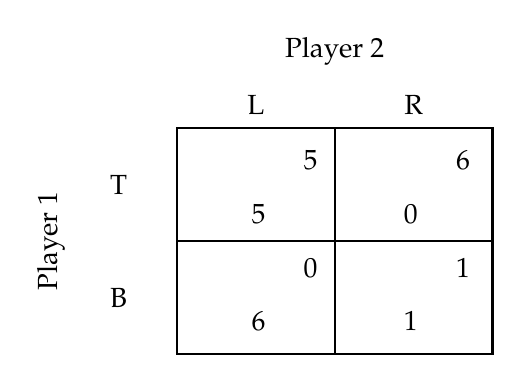
\begin{tikzpicture}
				\matrix[matrix of math nodes,
				every odd row/.style={align=right},every evenrow/.style={align=left},every node/.style={text width=1.5cm},row sep=0.2cm,column sep=0.2cm,ampersand replacement=\&] (m) {
					5\&6 \\
					5\&0 \\
					0 \&1 \\
					6 \&1\\
				};
				\draw (m.north east) rectangle (m.south west);
				\draw (m.north) -- (m.south);
				\draw (m.east) -- (m.west);
				
				% Player 1
				\coordinate (c) at ($(m.north west)!0.25!(m.south west)$);
				\coordinate (d) at ($(m.north west)!0.75!(m.south west)$);
				\node[left=2pt of c,text width=1cm]  {T};
				\node[left=2pt of d,text width=1cm]  {B};
				
				% Player 2
				\coordinate (a) at ($(m.north west)!0.25!(m.north east)$);
				\coordinate (b) at ($(m.north west)!0.75!(m.north east)$);
				\node[above=5pt of a,anchor=base] {L};
				\node[above=5pt of b,anchor=base] {R};
				
				\node[above=18pt of m.north] (firm b) {Player 2};
				\node[left=1.6cm of m.west,rotate=90,align=center,anchor=center] {Player 1};
				
				%\node[above=5pt of firm b]  {Payoff Matrix};
			\end{tikzpicture}
		\end{column}
	\end{columns}
\end{frame}

\begin{frame}{Repeated games}
	\begin{wideitemize}
		\item Why does the equilibrium in the repeated game differ from the one period game?
		\item \textbf{Because players can react to other players' past actions, repeated games allow for equilibrium outcomes that would not be an equilibrium in the corresponding one-shot game.}
		\item In this class, the main application of repeated games will be on collusive agreements. Many other economic examples (typically, when agents cannot sign an enforceable contract):
		\begin{wideitemize}
			\item Economic interactions when reputation is important
			\item International agreements (e.g. WTO, Kyoto)
			\item Informal economic relationships built on trust
		\end{wideitemize}
	\end{wideitemize}
\end{frame}

\begin{frame}{Repeated games: steps to solve}
		\begin{wideitemize}
			\item Steps to show that a particular strategy (e.g. grim trigger) is a Nash equilibrium
			\item 1. Find the payoff from the proposed equilibrium using the present discounted value formula
			\item 2. Find the payoff from \textit{unilaterally deviating} using the present discounted value formula
			\item 3. Determine whether the payoff from the proposed equilibrium is greater than the payoff from deviating. If the payoff is higher, then it is an equilibrium.
		\end{wideitemize}
\end{frame}

\begin{frame}{Repeated games: prisoner's dilemma with $T=\infty$}
	\begin{columns}[onlytextwidth, T] 
		\begin{column}{.55\textwidth}
			\begin{wideitemize}
				\item \textbf{Question:} For what discount values $\delta$ is the grim trigger strategy a Nash equilibrium in the following game?
			\end{wideitemize}
		\end{column}
		\begin{column}{.45\textwidth}
			\vspace{20pt}
			\hspace{20pt}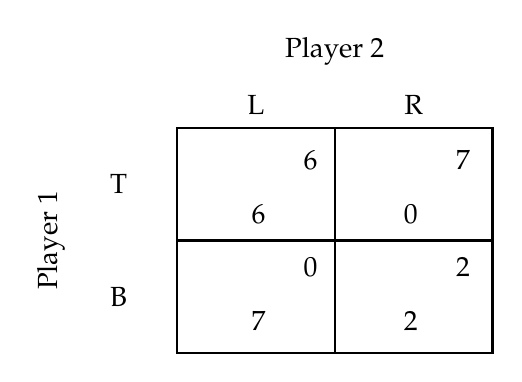
\begin{tikzpicture}
				\matrix[matrix of math nodes,
				every odd row/.style={align=right},every evenrow/.style={align=left},every node/.style={text width=1.5cm},row sep=0.2cm,column sep=0.2cm,ampersand replacement=\&] (m) {
					6\&7 \\
					6\&0 \\
					0 \&2 \\
					7 \&2\\
				};
				\draw (m.north east) rectangle (m.south west);
				\draw (m.north) -- (m.south);
				\draw (m.east) -- (m.west);
				
				% Player 1
				\coordinate (c) at ($(m.north west)!0.25!(m.south west)$);
				\coordinate (d) at ($(m.north west)!0.75!(m.south west)$);
				\node[left=2pt of c,text width=1cm]  {T};
				\node[left=2pt of d,text width=1cm]  {B};
				
				% Player 2
				\coordinate (a) at ($(m.north west)!0.25!(m.north east)$);
				\coordinate (b) at ($(m.north west)!0.75!(m.north east)$);
				\node[above=5pt of a,anchor=base] {L};
				\node[above=5pt of b,anchor=base] {R};
				
				\node[above=18pt of m.north] (firm b) {Player 2};
				\node[left=1.6cm of m.west,rotate=90,align=center,anchor=center] {Player 1};
				
				%\node[above=5pt of firm b]  {Payoff Matrix};
			\end{tikzpicture}
		\end{column}
	\end{columns}
\end{frame}

\begin{frame}{Plan}
	\begin{wideenumerate}
		\item Present discounted value
		\item Repeated games: method
		\item \textbf{Stability of collusive agreements}
	\end{wideenumerate}
\end{frame}

\begin{frame}{Stability of collusive agreements}
	\begin{wideitemize}
		\item \textbf{Setup (same as Bertrand):} 
		\begin{wideitemize}
			\item Homogeneous product. 
			\item Two firms with the same constant MC.
			\item Firms set prices simultaneously. If firms set the same price then they split demand equally. 
			\item Note: If game is played once $\rightarrow$ Bertrand equilibrium
		\end{wideitemize}
		\item \textbf{Question}: if game is played repeatedly for infinite periods with discount factor $\delta$, for what values of $\delta$ is the follow \textit{grim trigger strategy} an equilibrium?
		\begin{wideitemize}
			\item Set $p=p^M$ if $p=p^M$ in the past.
			\item Set $p=MC$ otherwise
		\end{wideitemize}
		\item (Note: there might be other Nash equilibria, but we'll just check this one.)
	\end{wideitemize}
\end{frame}

\begin{frame}{Stability of collusive agreements: solution}
	\begin{wideitemize}
		\item Equilibrium net present value:
		\item $\Pi=0.5 \pi^M + \delta 0.5 \pi^M  + \delta^2 0.5 \pi^M  + ... = 0.5 \pi^M \frac{1}{1-\delta}$
		\item Net present value from deviating (and undercutting the rival):
		\item $\Pi'=\pi^M+\underbrace{\delta 0 + \delta^2 0 + ...}_{\text{Punishment: revert back to marginal cost}} = \pi^M + \frac{0}{1-\delta}$
		\item Nash equilibrium condition: 
		\item $\Pi \geq \Pi'$, substituting in payoffs, $\delta \geq 0.5$.
		\item \textbf{Note:} if discount factor is sufficiently high, then there exists a NE of the repeated game where firms set the monopoly price every period under the `threat' that if any firm deviates, both firms revert to pricing at the marginal cost level forever.
	\end{wideitemize}
\end{frame}

\begin{frame}{Stability of collusive agreements: discount factor}
	\begin{wideitemize}
		\item Previous analysis: discount factor is very important to whether a collusive agreement will be successful
		\item (How much do you discount \$1 next period vs \$ today)
		\item But what is this discount factor exactly and why is it $\delta<1$? How might it differ across industries and what are the implications for collusive agreements?
	\end{wideitemize}
\end{frame}

\begin{frame}{Stability of collusive agreements: discount factor}
	\begin{wideitemize}
		\item One reason why $\delta < 1$: opportunity cost of time.
		\item  If interest rate is $r$ per period then an investor might use \$1 to gain \$(1+r) next period. Then:
		\begin{align*}
			\delta = \frac{1}{1+r}
		\end{align*}
		\item \pause What if $r$ is the annual rate but firms can change their prices $f$ times per year? Then:			\begin{align*}
			\delta = \frac{1}{1+r/f}
		\end{align*}
	\end{wideitemize}
\end{frame}

\begin{frame}{Stability of collusive agreements: discount factor}
	\begin{wideitemize}
		\item Another reason why $\delta < 1$: payoff in the future might not be received at all.
		\item E.g. Two pharmaceutical firms colluding. What if a third firm discovers an innovation (e.g. a superior drug) that would eliminate the market for the two firms? (This story is probably unlikely for some other industries like cement.)
		\item Let $h$ be the probability that the industry will cease to exist one period later. Then:
		\begin{align*}
				\delta = \frac{1-h}{1+r/f}
		\end{align*}
		\item \pause What if industry is growing at rate $g$? Then, profits in $t+1$ are $1+g$ greater than in period $t$. 
		\item Could model this with a discount factor:
		\begin{align*}
			\delta = \frac{(1+g)(1-h)}{1+r/f}
		\end{align*}
	\end{wideitemize}
\end{frame}

\begin{frame}{Stability of collusive agreements: discount factor}
	\begin{align*}
		\delta = \frac{(1+g)(1-h)}{1+r/f}
	\end{align*}
	\begin{wideitemize}
		\item \textbf{Collusion is normally easier to maintain when firms interact frequently and when the probability of industry continuation and growth is high.}
	\end{wideitemize}
\end{frame}

\begin{frame}{Summary of key points*}
	%\vspace{-20pt}
	\begin{wideitemize}
		\item Know how to compute the present discounted value given a discount factor
		\item Know what the grim trigger strategy is and how to check whether it is an equilibrium (and, alternatively, for what discount factors it is an equilibrium) 
		\item Know how different industries may have different discount factors (which can affect how stable collusive agreements are).
	\end{wideitemize}
	\vspace{20pt}
	*To clarify, all the material in the slides, problem sets, etc is assessable unless stated otherwise, but I hope this summary might be a useful place to start when studying the material.
\end{frame}

\end{document}
